\documentclass[aspectratio=169]{beamer}

\usepackage{amsmath,amssymb}
\usepackage{booktabs}
\usepackage{graphicx}
\usepackage{hyperref}

\graphicspath{{../../../phase_01_python_prototype/figures/}}

\usetheme{Madrid}
\usecolortheme{default}

\title[Phase 1 Review]{Phase 1 Review: Lightweight Spike-Based DOA Sector Inference for Embedded Edge AI}
\author{Hossein Molhem}
\institute{Kennesaw State University\\EE 6900 Special Topics: Embedded AI for Autonomous Robots}
\date{Research Review Presentation\\\today}

\begin{document}

\begin{frame}
\titlepage
\end{frame}

\begin{frame}{Presentation Roadmap}
\begin{enumerate}
    \item Motivation and problem definition
    \item Phase 1 signal-processing and inference pipeline
    \item Dataset and experimental design
    \item Baseline and LIF-inspired results
    \item Accuracy--latency interpretation
    \item Limitations and future work
\end{enumerate}
\begin{block}{Target duration}
This slide deck is designed for a 15--17 minute presentation.
\end{block}
\end{frame}

\begin{frame}{Motivation}
\begin{itemize}
    \item Embedded AI systems operate under compute, memory, energy, and latency constraints.
    \item Many edge-sensing problems have useful physics-based structure.
    \item Spike-based inference can represent information as sparse temporal events.
    \item The project asks whether array-processing features can support spike-based temporal inference.
\end{itemize}
\end{frame}

\begin{frame}{Problem Statement}
\begin{block}{Phase 1 Question}
Can compact beamspace features extracted from a physics-based ULA signal model be converted into sparse spike trains and classified with acceptable accuracy and controllable temporal latency?
\end{block}
\vspace{0.2cm}
\begin{itemize}
    \item Task: four-class DOA sector classification.
    \item Scope: one narrowband source, controlled SNR grid.
    \item Purpose: establish a reproducible embedded-AI baseline, not a new high-resolution DOA estimator.
\end{itemize}
\end{frame}

\begin{frame}{Why DOA Sector Inference?}
\begin{itemize}
    \item DOA processing connects electromagnetics, radar, MIMO sensing, and array signal processing.
    \item Sector classification is smaller and more controlled than continuous-angle estimation.
    \item Beamspace features provide compact angular signatures.
    \item The covariance stage creates a natural bridge toward FPGA/HLS acceleration.
\end{itemize}
\end{frame}

\begin{frame}{End-to-End Phase 1 Pipeline}
\centering
\begin{tabular}{c}
ULA / DOA signal model \\
$\Downarrow$ \\
Array snapshots with controlled SNR \\
$\Downarrow$ \\
Sample covariance matrix $R_{xx}$ \\
$\Downarrow$ \\
Beamspace energy features \\
$\Downarrow$ \\
Nearest-centroid baseline \\
$\Downarrow$ \\
Rate-based spike encoding and LIF-inspired inference
\end{tabular}
\end{frame}

\begin{frame}{Theoretical Foundation}
\small
\begin{align*}
    a(\theta) &= [1,e^{-jkd\sin\theta},\ldots,e^{-j(N-1)kd\sin\theta}]^{T} \\
    R_{xx} &= \frac{1}{M}XX^{H} \\
    p(\phi) &= b^{H}(\phi)R_{xx}b(\phi) \\
    \hat{c} &= \arg\min_c \lVert x-\mu_c\rVert_2^2 \\
    v_c[t] &= \alpha v_c[t-1]+i_c[t]
\end{align*}
\begin{itemize}
    \item Covariance captures spatial correlation.
    \item Beamspace energy compresses spatial information.
    \item LIF accumulation creates a temporal decision process.
\end{itemize}
\end{frame}

\begin{frame}{Dataset Configuration}
\centering
\begin{tabular}{ll}
\toprule
Parameter & Value \\
\midrule
Array type & Uniform Linear Array \\
Array elements & 8 \\
Snapshots per sample & 128 \\
Element spacing & $\lambda/2$ \\
Source count & 1 \\
DOA range & $-60^{\circ}$ to $+60^{\circ}$ \\
DOA sectors & 4 \\
SNR values & $-10,-5,0,5,10,15,20$ dB \\
Total samples & 2800 \\
Test samples & 840 \\
\bottomrule
\end{tabular}
\end{frame}

\begin{frame}{Beamspace Feature Example}
\centering
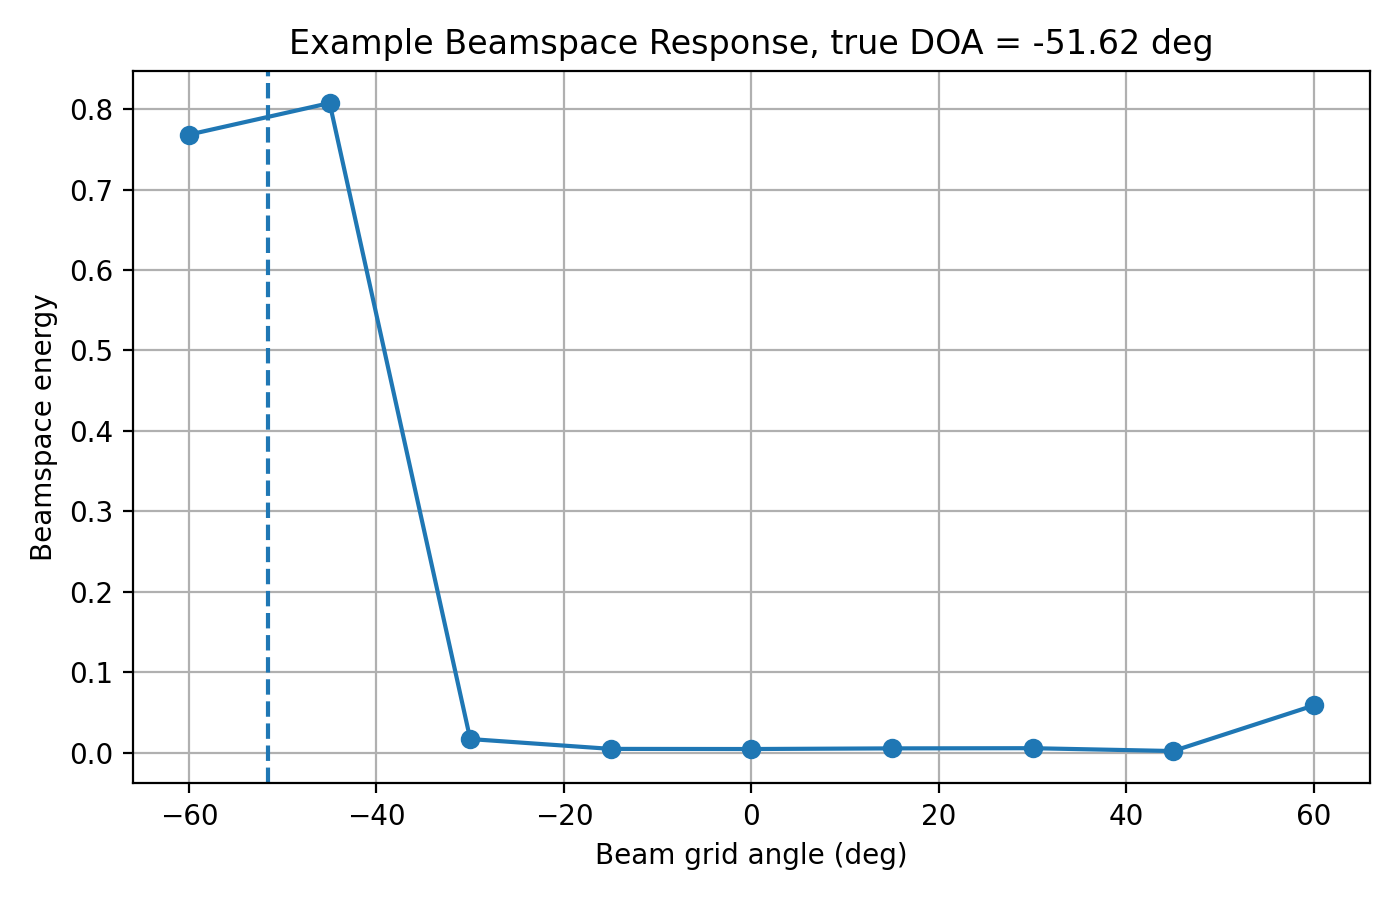
\includegraphics[width=0.78\linewidth]{run_001_example_beamspace_response.png}
\vspace{0.1cm}

\small Beamspace features provide compact angular information for coarse DOA-sector classification.
\end{frame}

\begin{frame}{Baseline Classifier}
\begin{block}{Nearest-centroid decision rule}
\[
    \hat{c}=\arg\min_c \lVert x-\mu_c\rVert_2^2
\]
\end{block}
\begin{itemize}
    \item Uses continuous normalized beamspace features.
    \item Deterministic, simple, and interpretable.
    \item Establishes the non-spiking reference accuracy.
    \item Overall test accuracy: $0.869048$ or $86.90\%$.
\end{itemize}
\end{frame}

\begin{frame}{Spike Encoding and LIF-Inspired Inference}
\begin{columns}
\column{0.48\textwidth}
\textbf{Rate-based spike encoding}
\begin{itemize}
    \item Normalized feature values become spike probabilities.
    \item Larger features generate more spikes over time.
    \item Produces sparse temporal representations.
\end{itemize}
\column{0.48\textwidth}
\textbf{LIF-inspired classifier}
\begin{itemize}
    \item Class-level membrane evidence.
    \item Leak controls evidence retention.
    \item Stable-decision latency becomes measurable.
\end{itemize}
\end{columns}
\end{frame}

\begin{frame}{Fixed LIF Configuration}
\begin{equation*}
    v_c[t] = \alpha v_c[t-1] + i_c[t]
\end{equation*}
\begin{block}{Run 003}
\centering
$T=20$, leak $=0.97$\\
Accuracy $=0.825000$\\
Mean stable-decision latency $=6.423810$ time steps
\end{block}
\begin{itemize}
    \item The fixed LIF path preserves useful classification behavior.
    \item It remains below the continuous baseline in raw accuracy.
\end{itemize}
\end{frame}

\begin{frame}{Accuracy Comparison Versus SNR}
\centering
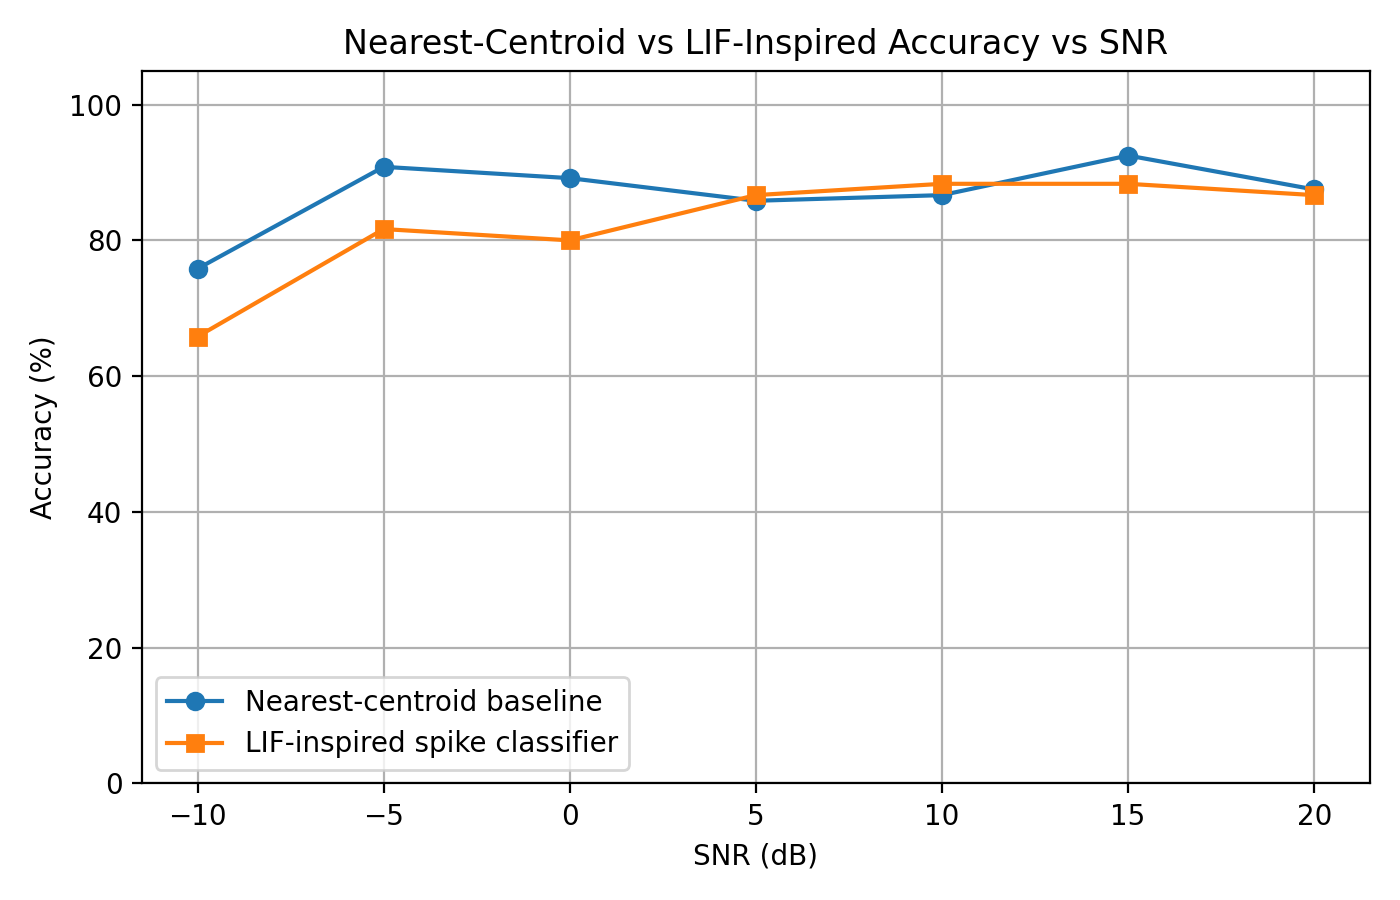
\includegraphics[width=0.82\linewidth]{run_004_accuracy_comparison_vs_snr.png}
\vspace{0.1cm}

\small The continuous baseline remains stronger, but the LIF path retains useful sector information.
\end{frame}

\begin{frame}{Stable-Decision Latency Versus SNR}
\centering
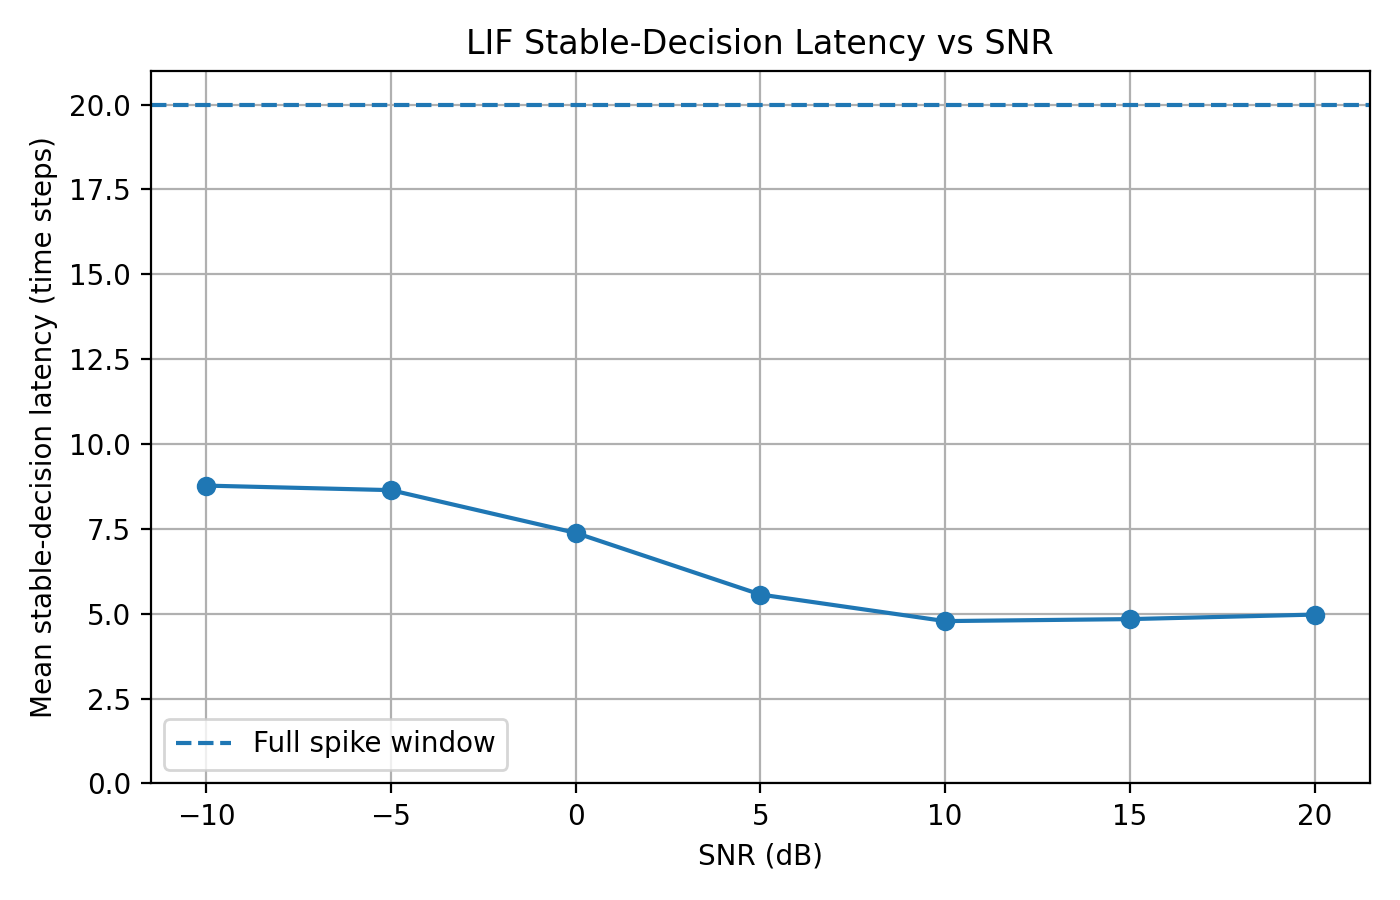
\includegraphics[width=0.82\linewidth]{run_004_lif_latency_vs_snr.png}
\vspace{0.1cm}

\small Higher signal quality generally supports earlier stabilization of the temporal decision.
\end{frame}

\begin{frame}{Run 005 Parameter Sweep}
\centering
\begin{tabular}{lrrrr}
\toprule
Case & $T$ & Leak & Accuracy & Latency \\
\midrule
Best LIF accuracy & 40 & 0.99 & 0.841667 & 8.396429 \\
Lowest latency & 10 & 0.99 & 0.776190 & 3.782143 \\
Fixed Run 003 & 20 & 0.97 & 0.825000 & 6.423810 \\
Baseline & -- & -- & 0.869048 & -- \\
\bottomrule
\end{tabular}
\vspace{0.3cm}

\small The sweep exposes a tunable accuracy--latency design space.
\end{frame}

\begin{frame}{Accuracy--Latency Trade-Off}
\centering
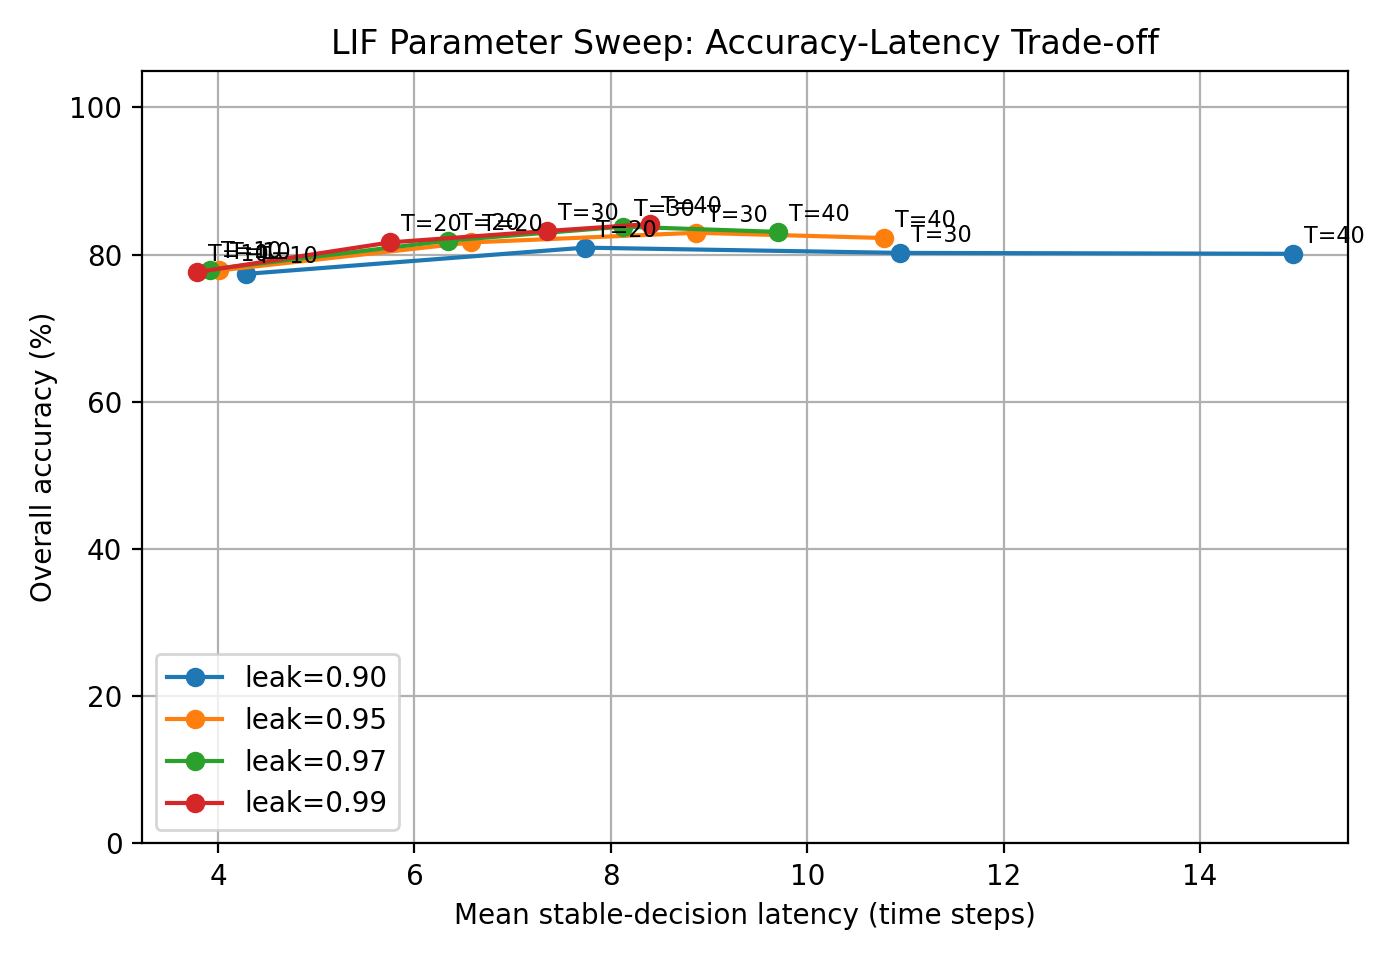
\includegraphics[width=0.80\linewidth]{run_005_lif_accuracy_latency_tradeoff.png}
\vspace{0.1cm}

\small Longer spike windows and stronger evidence retention generally improve accuracy but increase the temporal budget.
\end{frame}

\begin{frame}{Main Engineering Interpretation}
\begin{itemize}
    \item The spike-based path does not improve raw accuracy over the continuous nearest-centroid baseline.
    \item This is an expected and useful result because rate-based spikes introduce stochastic quantization.
    \item The value of the spike path is architectural:
    \begin{itemize}
        \item sparse temporal inference,
        \item measurable stable-decision latency,
        \item tunable accuracy--latency behavior.
    \end{itemize}
\end{itemize}
\end{frame}

\begin{frame}{Connection to Prior FPGA/HLS SCM Work}
\begin{itemize}
    \item Prior work implemented a Vitis HLS sample-covariance-matrix accelerator for DOA preprocessing.
    \item That project targets the covariance stage:
    \[
        R_{xx}=\frac{1}{M}XX^{H}
    \]
    \item The current Embedded AI project builds on the same covariance-based DOA foundation.
    \item Together, the two repositories create a path from DOA preprocessing to hardware-aware spike-based inference.
\end{itemize}
\end{frame}

\begin{frame}{Limitations}
\begin{itemize}
    \item Single-source narrowband ULA model.
    \item Sector classification rather than continuous high-resolution DOA estimation.
    \item Rate-based spike encoding introduces stochastic variation.
    \item LIF classifier is a simplified class-level temporal accumulator.
    \item Current implementation is Python-based and not yet fixed-point or deployed on FPGA.
\end{itemize}
\end{frame}

\begin{frame}{Conclusion and Future Work}
\begin{block}{Conclusion}
Phase 1 establishes a reproducible DOA-sector embedded-AI baseline. The continuous beamspace classifier provides strong accuracy, while the spike-based path provides sparse temporal inference and explicit latency control.
\end{block}
\begin{itemize}
    \item Baseline accuracy: $86.90\%$.
    \item Best LIF accuracy: $84.17\%$.
    \item Next steps: richer DOA cases, fixed-point analysis, PYNQ/Vitis HLS refactoring, and hardware-aware deployment planning.
\end{itemize}
\end{frame}

\begin{frame}{Closing Message}
\centering
\Large
Phase 1 converts a physics-based DOA feature pipeline into a latency-aware embedded-AI inference baseline.

\vspace{0.5cm}
\normalsize
The main contribution is not higher raw accuracy; it is a controlled bridge toward sparse temporal and hardware-aware edge inference.
\end{frame}

\end{document}
